%------------------------------------------------------------------------------------------------------------------------------------------------------
% Reiniciar numeração das figuras que aparecem no apêndice
\setcounter{figure}{0}
\setcounter{table}{0}

\chapter{Circuito}
\label{apend:circ}
\vspace{-1.9cm}
\newcommand\measurepage{\dimexpr\pagegoal-\pagetotal-\baselineskip\relax}
\begin{figure}[H]
  \setlength{\abovecaptionskip}{0pt}
  \setlength{\belowcaptionskip}{0pt}
  \caption[Diagrama do circuito elétrico]{Diagrama do circuito elétrico}
  \centering
  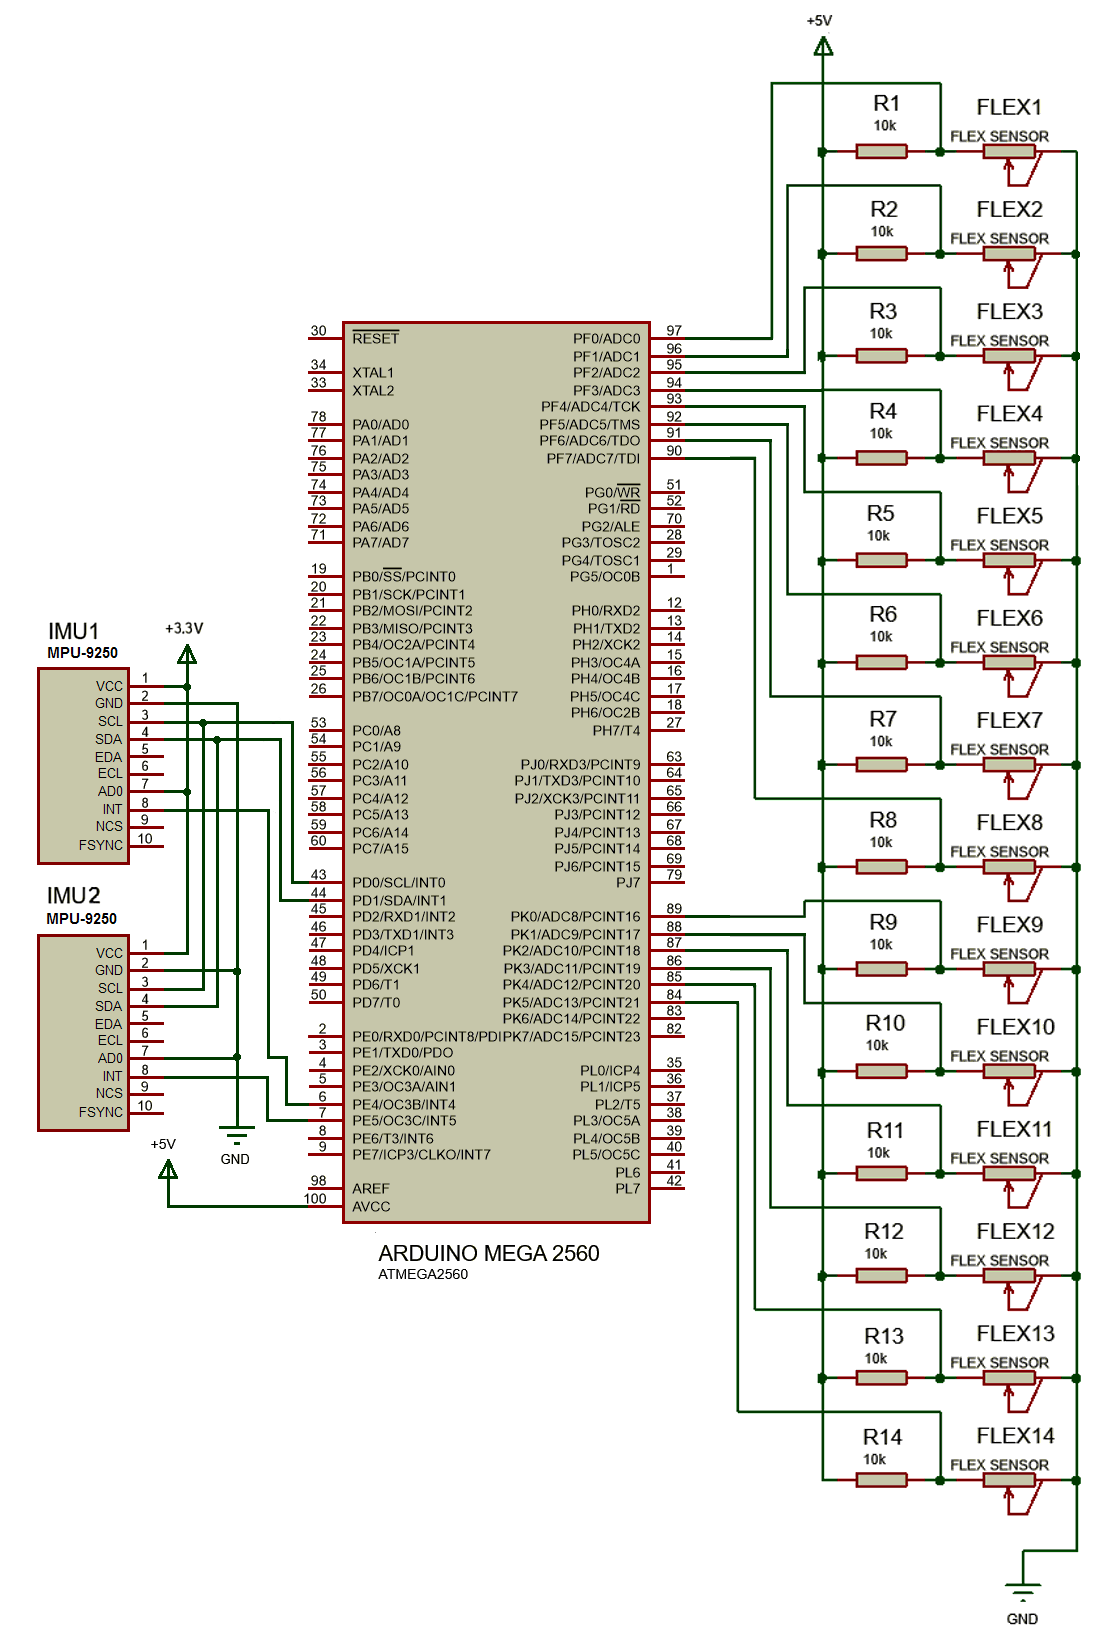
\includegraphics[height=\measurepage,width=\textwidth,keepaspectratio]{imagem/Circuito_Rotacionado}
  \captionsetup{justification=centering}
  \captionfont{\small{\textbf{\\Fonte: Elaborado pelo autor (2016)}}}
  \label{fig:circuito}
\end{figure}

\chapter{Código Arduino}
\label{apend:codigoArd}
\vspace{-1.9cm}

Textos ou documentos elaborados pelo autor, como por exemplo código-fonte.

\lstinputlisting[language=C++, label=lst:codigoArduino, caption={Trecho de código modificado},morekeywords={ResponsiveAnalogRead,MPU9250,delay,Serial,begin,println,print,attachInterrupt,pinMode,Quaternion}]{pos-texto/TCC_Arduino.ino}

\chapter{Código Unity}
\label{apend:codigoUni}
\vspace{-1.9cm}

Textos ou documentos elaborados pelo autor, como por exemplo código-fonte.

\lstinputlisting[language={[Sharp]C}, label=lst:codigoUnity, caption={Trecho de código modificado},morekeywords={SerialPort,IsOpen,Close,Open,Quaternion,GameObject,Vector3,Split,transform,localEulerAngles,Parse,Set,eulerAngles,x,y,z}]{pos-texto/Rotator2.cs}
